\section{代码}

\begin{PythonCode}\label{例1}
	\begin{Verbatim}[commandchars=\\\{\}]
\PY{c+c1}{\PYZsh{} 导入操作系统库}
\PY{k+kn}{import} \PY{n+nn}{os}
\PY{c+c1}{\PYZsh{} 更改工作目录}
\PY{n}{os}\PY{o}{.}\PY{n}{chdir}\PY{p}{(}\PY{l+s+sa}{r}\PY{l+s+s2}{\PYZdq{}}\PY{l+s+s2}{D:}\PY{l+s+s2}{\PYZbs{}}\PY{l+s+s2}{softwares}\PY{l+s+s2}{\PYZbs{}}\PY{l+s+s2}{applied statistics}\PY{l+s+s2}{\PYZbs{}}\PY{l+s+s2}{pythoncodelearning}\PY{l+s+s2}{\PYZbs{}}\PY{l+s+s2}{chap8}\PY{l+s+s2}{\PYZbs{}}\PY{l+s+s2}{sourcecode}\PY{l+s+s2}{\PYZdq{}}\PY{p}{)}
\PY{c+c1}{\PYZsh{} 导入基础计算库}
\PY{k+kn}{import} \PY{n+nn}{numpy} \PY{k}{as} \PY{n+nn}{np}
\PY{c+c1}{\PYZsh{} 导入绘图库}
\PY{k+kn}{import} \PY{n+nn}{matplotlib}\PY{n+nn}{.}\PY{n+nn}{pyplot} \PY{k}{as} \PY{n+nn}{plt}
\PY{c+c1}{\PYZsh{} 导入数据划分工具}
\PY{k+kn}{from} \PY{n+nn}{sklearn}\PY{n+nn}{.}\PY{n+nn}{model\PYZus{}selection} \PY{k+kn}{import} \PY{n}{train\PYZus{}test\PYZus{}split}
\PY{c+c1}{\PYZsh{} 导入Gassian朴素贝叶斯分类器}
\PY{k+kn}{from} \PY{n+nn}{sklearn}\PY{n+nn}{.}\PY{n+nn}{naive\PYZus{}bayes} \PY{k+kn}{import} \PY{n}{GaussianNB}
\PY{c+c1}{\PYZsh{} 导入数据获取工具}
\PY{k+kn}{from} \PY{n+nn}{sklearn}\PY{n+nn}{.}\PY{n+nn}{datasets} \PY{k+kn}{import} \PY{n}{load\PYZus{}iris}
\PY{c+c1}{\PYZsh{} 导入绘图库中的字体管理包}
\PY{k+kn}{from} \PY{n+nn}{matplotlib} \PY{k+kn}{import} \PY{n}{font\PYZus{}manager}
\PY{c+c1}{\PYZsh{} 实现中文字符正常显示}
\PY{n}{font} \PY{o}{=} \PY{n}{font\PYZus{}manager}\PY{o}{.}\PY{n}{FontProperties}\PY{p}{(}\PY{n}{fname}\PY{o}{=}\PY{l+s+sa}{r}\PY{l+s+s2}{\PYZdq{}}\PY{l+s+s2}{C:}\PY{l+s+s2}{\PYZbs{}}\PY{l+s+s2}{Windows}\PY{l+s+s2}{\PYZbs{}}\PY{l+s+s2}{Fonts}\PY{l+s+s2}{\PYZbs{}}\PY{l+s+s2}{SimKai.ttf}\PY{l+s+s2}{\PYZdq{}}\PY{p}{)}
\PY{c+c1}{\PYZsh{} 使用seaborn风格绘图}
\PY{n}{plt}\PY{o}{.}\PY{n}{style}\PY{o}{.}\PY{n}{use}\PY{p}{(}\PY{l+s+s2}{\PYZdq{}}\PY{l+s+s2}{seaborn\PYZhy{}v0\PYZus{}8}\PY{l+s+s2}{\PYZdq{}}\PY{p}{)}
\PY{c+c1}{\PYZsh{} 获取数据}
\PY{n}{X}\PY{p}{,} \PY{n}{y} \PY{o}{=} \PY{n}{load\PYZus{}iris}\PY{p}{(}\PY{n}{return\PYZus{}X\PYZus{}y}\PY{o}{=}\PY{k+kc}{True}\PY{p}{)}
\PY{c+c1}{\PYZsh{} 数据划分}
\PY{n}{X\PYZus{}train}\PY{p}{,} \PY{n}{X\PYZus{}test}\PY{p}{,} \PY{n}{y\PYZus{}train}\PY{p}{,} \PY{n}{y\PYZus{}test} \PY{o}{=} \PY{n}{train\PYZus{}test\PYZus{}split}\PY{p}{(}
    \PY{n}{X}\PY{p}{,} \PY{n}{y}\PY{p}{,} \PY{n}{test\PYZus{}size}\PY{o}{=}\PY{l+m+mf}{0.5}\PY{p}{,} \PY{n}{random\PYZus{}state}\PY{o}{=}\PY{l+m+mi}{0}
\PY{p}{)}
\PY{c+c1}{\PYZsh{} 构建模型}
\PY{n}{gnb} \PY{o}{=} \PY{n}{GaussianNB}\PY{p}{(}\PY{p}{)}
\PY{c+c1}{\PYZsh{} 模型拟合}
\PY{n}{gnb}\PY{o}{.}\PY{n}{fit}\PY{p}{(}\PY{n}{X\PYZus{}train}\PY{p}{,} \PY{n}{y\PYZus{}train}\PY{p}{)}
\PY{c+c1}{\PYZsh{} 预测}
\PY{n}{y\PYZus{}pred} \PY{o}{=} \PY{n}{gnb}\PY{o}{.}\PY{n}{predict}\PY{p}{(}\PY{n}{X\PYZus{}test}\PY{p}{)}
\PY{n+nb}{print}\PY{p}{(}\PY{n}{y\PYZus{}pred}\PY{p}{[}\PY{l+m+mi}{1}\PY{p}{:}\PY{l+m+mi}{5}\PY{p}{]}\PY{p}{)}
\PY{c+c1}{\PYZsh{} 分类准确率}
\PY{n}{corrate} \PY{o}{=} \PY{n}{np}\PY{o}{.}\PY{n}{mean}\PY{p}{(}\PY{n}{y\PYZus{}pred}\PY{o}{==}\PY{n}{y\PYZus{}test}\PY{p}{)}
\PY{n+nb}{print}\PY{p}{(}\PY{l+s+s2}{\PYZdq{}}\PY{l+s+s2}{分类准确率为:}\PY{l+s+s2}{\PYZdq{}}\PY{p}{)}
\PY{n+nb}{print}\PY{p}{(}\PY{n}{corrate}\PY{p}{)}
\end{Verbatim}

\begin{Verbatim}[commandchars=\\\{\}]
[1 0 2 0]
分类准确率为:
0.9466666666666667
\end{Verbatim}
\end{PythonCode}

\begin{figure}
	\centering
	\includegraphics[width=14cm]{codeimage/code1}
	\caption{code1}
	\label{code1}
\end{figure}

\begin{PythonCode}\label{例2}
	\begin{Verbatim}[commandchars=\\\{\}]
\PY{c+c1}{\PYZsh{} 导入操作系统库}
\PY{k+kn}{import} \PY{n+nn}{os}
\PY{c+c1}{\PYZsh{} 更改工作目录}
\PY{n}{os}\PY{o}{.}\PY{n}{chdir}\PY{p}{(}\PY{l+s+sa}{r}\PY{l+s+s2}{\PYZdq{}}\PY{l+s+s2}{D:}\PY{l+s+s2}{\PYZbs{}}\PY{l+s+s2}{softwares}\PY{l+s+s2}{\PYZbs{}}\PY{l+s+s2}{applied statistics}\PY{l+s+s2}{\PYZbs{}}\PY{l+s+s2}{pythoncodelearning}\PY{l+s+s2}{\PYZbs{}}\PY{l+s+s2}{chap2}\PY{l+s+s2}{\PYZbs{}}\PY{l+s+s2}{sourcecode}\PY{l+s+s2}{\PYZdq{}}\PY{p}{)}
\PY{c+c1}{\PYZsh{} 导入绘图库}
\PY{k+kn}{import} \PY{n+nn}{matplotlib}\PY{n+nn}{.}\PY{n+nn}{pyplot} \PY{k}{as} \PY{n+nn}{plt}
\PY{k+kn}{import} \PY{n+nn}{matplotlib} \PY{k}{as} \PY{n+nn}{mpl}
\PY{c+c1}{\PYZsh{} 导入线性和二次判别分析工具}
\PY{k+kn}{from} \PY{n+nn}{sklearn}\PY{n+nn}{.}\PY{n+nn}{discriminant\PYZus{}analysis} \PY{k+kn}{import} \PY{n}{LinearDiscriminantAnalysis}
\PY{c+c1}{\PYZsh{} 加载数据集}
\PY{k+kn}{from} \PY{n+nn}{sklearn}\PY{n+nn}{.}\PY{n+nn}{datasets} \PY{k+kn}{import} \PY{n}{load\PYZus{}iris}
\PY{c+c1}{\PYZsh{} 导入PCA工具}
\PY{k+kn}{from} \PY{n+nn}{sklearn}\PY{n+nn}{.}\PY{n+nn}{decomposition} \PY{k+kn}{import} \PY{n}{PCA}
\PY{c+c1}{\PYZsh{} 导入绘图库中的字体管理包}
\PY{k+kn}{from} \PY{n+nn}{matplotlib} \PY{k+kn}{import} \PY{n}{font\PYZus{}manager}
\PY{c+c1}{\PYZsh{} 实现中文字符正常显示}
\PY{n}{font} \PY{o}{=} \PY{n}{font\PYZus{}manager}\PY{o}{.}\PY{n}{FontProperties}\PY{p}{(}\PY{n}{fname}\PY{o}{=}\PY{l+s+sa}{r}\PY{l+s+s2}{\PYZdq{}}\PY{l+s+s2}{C:}\PY{l+s+s2}{\PYZbs{}}\PY{l+s+s2}{Windows}\PY{l+s+s2}{\PYZbs{}}\PY{l+s+s2}{Fonts}\PY{l+s+s2}{\PYZbs{}}\PY{l+s+s2}{SimKai.ttf}\PY{l+s+s2}{\PYZdq{}}\PY{p}{)}
\PY{c+c1}{\PYZsh{} 使用seaborn风格绘图}
\PY{n}{plt}\PY{o}{.}\PY{n}{style}\PY{o}{.}\PY{n}{use}\PY{p}{(}\PY{l+s+s2}{\PYZdq{}}\PY{l+s+s2}{seaborn\PYZhy{}v0\PYZus{}8}\PY{l+s+s2}{\PYZdq{}}\PY{p}{)}
\PY{c+c1}{\PYZsh{} 加载数据集}
\PY{n}{iris} \PY{o}{=} \PY{n}{load\PYZus{}iris}\PY{p}{(}\PY{p}{)}
\PY{n}{X} \PY{o}{=} \PY{n}{iris}\PY{o}{.}\PY{n}{data}
\PY{n}{y} \PY{o}{=} \PY{n}{iris}\PY{o}{.}\PY{n}{target}
\PY{n}{target\PYZus{}names} \PY{o}{=} \PY{n}{iris}\PY{o}{.}\PY{n}{target\PYZus{}names}
\PY{c+c1}{\PYZsh{} 建立PCA模型,指定两个主成分}
\PY{n}{pca} \PY{o}{=} \PY{n}{PCA}\PY{p}{(}\PY{n}{n\PYZus{}components}\PY{o}{=}\PY{l+m+mi}{2}\PY{p}{)}
\PY{c+c1}{\PYZsh{} 模型拟合}
\PY{n}{pca}\PY{o}{.}\PY{n}{fit}\PY{p}{(}\PY{n}{X}\PY{p}{)}
\PY{c+c1}{\PYZsh{} 主成分的值}
\PY{n}{X\PYZus{}r} \PY{o}{=} \PY{n}{pca}\PY{o}{.}\PY{n}{transform}\PY{p}{(}\PY{n}{X}\PY{p}{)}
\PY{c+c1}{\PYZsh{} 建立LDA模型,两个主成分}
\PY{n}{lda} \PY{o}{=} \PY{n}{LinearDiscriminantAnalysis}\PY{p}{(}\PY{n}{n\PYZus{}components}\PY{o}{=}\PY{l+m+mi}{2}\PY{p}{)}
\PY{c+c1}{\PYZsh{} 模型拟合}
\PY{n}{lda}\PY{o}{.}\PY{n}{fit}\PY{p}{(}\PY{n}{X}\PY{p}{,} \PY{n}{y}\PY{p}{)}
\PY{c+c1}{\PYZsh{} 计算主成分的值}
\PY{n}{X\PYZus{}r2} \PY{o}{=} \PY{n}{lda}\PY{o}{.}\PY{n}{transform}\PY{p}{(}\PY{n}{X}\PY{p}{)}
\PY{c+c1}{\PYZsh{} 方差解释比}
\PY{n+nb}{print}\PY{p}{(}
    \PY{l+s+s2}{\PYZdq{}}\PY{l+s+s2}{explained variance ratio (first two components): }\PY{l+s+si}{\PYZpc{}s}\PY{l+s+s2}{\PYZdq{}}
    \PY{o}{\PYZpc{}} \PY{n+nb}{str}\PY{p}{(}\PY{n}{pca}\PY{o}{.}\PY{n}{explained\PYZus{}variance\PYZus{}ratio\PYZus{}}\PY{p}{)}
\PY{p}{)}
\PY{c+c1}{\PYZsh{} 开始绘图}
\PY{n}{fig1}\PY{p}{,} \PY{n}{ax} \PY{o}{=} \PY{n}{plt}\PY{o}{.}\PY{n}{subplots}\PY{p}{(}\PY{n}{figsize}\PY{o}{=}\PY{p}{(}\PY{l+m+mi}{6}\PY{p}{,}\PY{l+m+mi}{6}\PY{p}{)}\PY{p}{)}
\PY{n}{colors} \PY{o}{=} \PY{p}{[}\PY{l+s+s2}{\PYZdq{}}\PY{l+s+s2}{navy}\PY{l+s+s2}{\PYZdq{}}\PY{p}{,} \PY{l+s+s2}{\PYZdq{}}\PY{l+s+s2}{turquoise}\PY{l+s+s2}{\PYZdq{}}\PY{p}{,} \PY{l+s+s2}{\PYZdq{}}\PY{l+s+s2}{darkorange}\PY{l+s+s2}{\PYZdq{}}\PY{p}{]}
\PY{n}{lw} \PY{o}{=} \PY{l+m+mi}{2}
\PY{k}{for} \PY{n}{color}\PY{p}{,} \PY{n}{i}\PY{p}{,} \PY{n}{target\PYZus{}name} \PY{o+ow}{in} \PY{n+nb}{zip}\PY{p}{(}\PY{n}{colors}\PY{p}{,} \PY{p}{[}\PY{l+m+mi}{0}\PY{p}{,} \PY{l+m+mi}{1}\PY{p}{,} \PY{l+m+mi}{2}\PY{p}{]}\PY{p}{,} \PY{n}{target\PYZus{}names}\PY{p}{)}\PY{p}{:}
    \PY{n}{ax}\PY{o}{.}\PY{n}{scatter}\PY{p}{(}
        \PY{n}{X\PYZus{}r}\PY{p}{[}\PY{n}{y} \PY{o}{==} \PY{n}{i}\PY{p}{,} \PY{l+m+mi}{0}\PY{p}{]}\PY{p}{,} \PY{c+c1}{\PYZsh{} 第一主成分,分类别}
        \PY{n}{X\PYZus{}r}\PY{p}{[}\PY{n}{y} \PY{o}{==} \PY{n}{i}\PY{p}{,} \PY{l+m+mi}{1}\PY{p}{]}\PY{p}{,} \PY{c+c1}{\PYZsh{} 第二主成分,分类别}
        \PY{n}{color}\PY{o}{=}\PY{n}{color}\PY{p}{,} \PY{n}{alpha}\PY{o}{=}\PY{l+m+mf}{0.8}\PY{p}{,} 
        \PY{n}{lw}\PY{o}{=}\PY{n}{lw}\PY{p}{,} \PY{n}{label}\PY{o}{=}\PY{n}{target\PYZus{}name}
    \PY{p}{)}
\PY{n}{ax}\PY{o}{.}\PY{n}{legend}\PY{p}{(}\PY{n}{loc}\PY{o}{=}\PY{l+s+s2}{\PYZdq{}}\PY{l+s+s2}{best}\PY{l+s+s2}{\PYZdq{}}\PY{p}{,} \PY{n}{shadow}\PY{o}{=}\PY{k+kc}{False}\PY{p}{,} \PY{n}{scatterpoints}\PY{o}{=}\PY{l+m+mi}{1}\PY{p}{)}
\PY{n}{ax}\PY{o}{.}\PY{n}{set\PYZus{}title}\PY{p}{(}\PY{l+s+s2}{\PYZdq{}}\PY{l+s+s2}{PCA of IRIS dataset}\PY{l+s+s2}{\PYZdq{}}\PY{p}{)}
\PY{n}{plt}\PY{o}{.}\PY{n}{show}\PY{p}{(}\PY{p}{)}
\PY{n}{fig1}\PY{o}{.}\PY{n}{savefig}\PY{p}{(}\PY{l+s+s2}{\PYZdq{}}\PY{l+s+s2}{../codeimage/code2.pdf}\PY{l+s+s2}{\PYZdq{}}\PY{p}{)}

\PY{n}{fig2}\PY{p}{,} \PY{n}{ax} \PY{o}{=} \PY{n}{plt}\PY{o}{.}\PY{n}{subplots}\PY{p}{(}\PY{n}{figsize}\PY{o}{=}\PY{p}{(}\PY{l+m+mi}{6}\PY{p}{,}\PY{l+m+mi}{6}\PY{p}{)}\PY{p}{)}
\PY{k}{for} \PY{n}{color}\PY{p}{,} \PY{n}{i}\PY{p}{,} \PY{n}{target\PYZus{}name} \PY{o+ow}{in} \PY{n+nb}{zip}\PY{p}{(}\PY{n}{colors}\PY{p}{,} \PY{p}{[}\PY{l+m+mi}{0}\PY{p}{,} \PY{l+m+mi}{1}\PY{p}{,} \PY{l+m+mi}{2}\PY{p}{]}\PY{p}{,} \PY{n}{target\PYZus{}names}\PY{p}{)}\PY{p}{:}
    \PY{n}{ax}\PY{o}{.}\PY{n}{scatter}\PY{p}{(}
        \PY{n}{X\PYZus{}r2}\PY{p}{[}\PY{n}{y} \PY{o}{==} \PY{n}{i}\PY{p}{,} \PY{l+m+mi}{0}\PY{p}{]}\PY{p}{,} 
        \PY{n}{X\PYZus{}r2}\PY{p}{[}\PY{n}{y} \PY{o}{==} \PY{n}{i}\PY{p}{,} \PY{l+m+mi}{1}\PY{p}{]}\PY{p}{,} 
        \PY{n}{alpha}\PY{o}{=}\PY{l+m+mf}{0.8}\PY{p}{,} \PY{n}{color}\PY{o}{=}\PY{n}{color}\PY{p}{,} 
        \PY{n}{label}\PY{o}{=}\PY{n}{target\PYZus{}name}
    \PY{p}{)}
\PY{n}{ax}\PY{o}{.}\PY{n}{legend}\PY{p}{(}\PY{n}{loc}\PY{o}{=}\PY{l+s+s2}{\PYZdq{}}\PY{l+s+s2}{best}\PY{l+s+s2}{\PYZdq{}}\PY{p}{,} \PY{n}{shadow}\PY{o}{=}\PY{k+kc}{False}\PY{p}{,} \PY{n}{scatterpoints}\PY{o}{=}\PY{l+m+mi}{1}\PY{p}{)}
\PY{n}{ax}\PY{o}{.}\PY{n}{set\PYZus{}title}\PY{p}{(}\PY{l+s+s2}{\PYZdq{}}\PY{l+s+s2}{LDA of IRIS dataset}\PY{l+s+s2}{\PYZdq{}}\PY{p}{)}
\PY{n}{plt}\PY{o}{.}\PY{n}{show}\PY{p}{(}\PY{p}{)}
\PY{n}{fig2}\PY{o}{.}\PY{n}{savefig}\PY{p}{(}\PY{l+s+s2}{\PYZdq{}}\PY{l+s+s2}{../codeimage/code3.pdf}\PY{l+s+s2}{\PYZdq{}}\PY{p}{)}
\end{Verbatim}

\begin{Verbatim}[commandchars=\\\{\}]
explained variance ratio (first two components): [0.92461872 0.05306648]
\end{Verbatim}
\end{PythonCode}

\begin{figure}
	\centering
	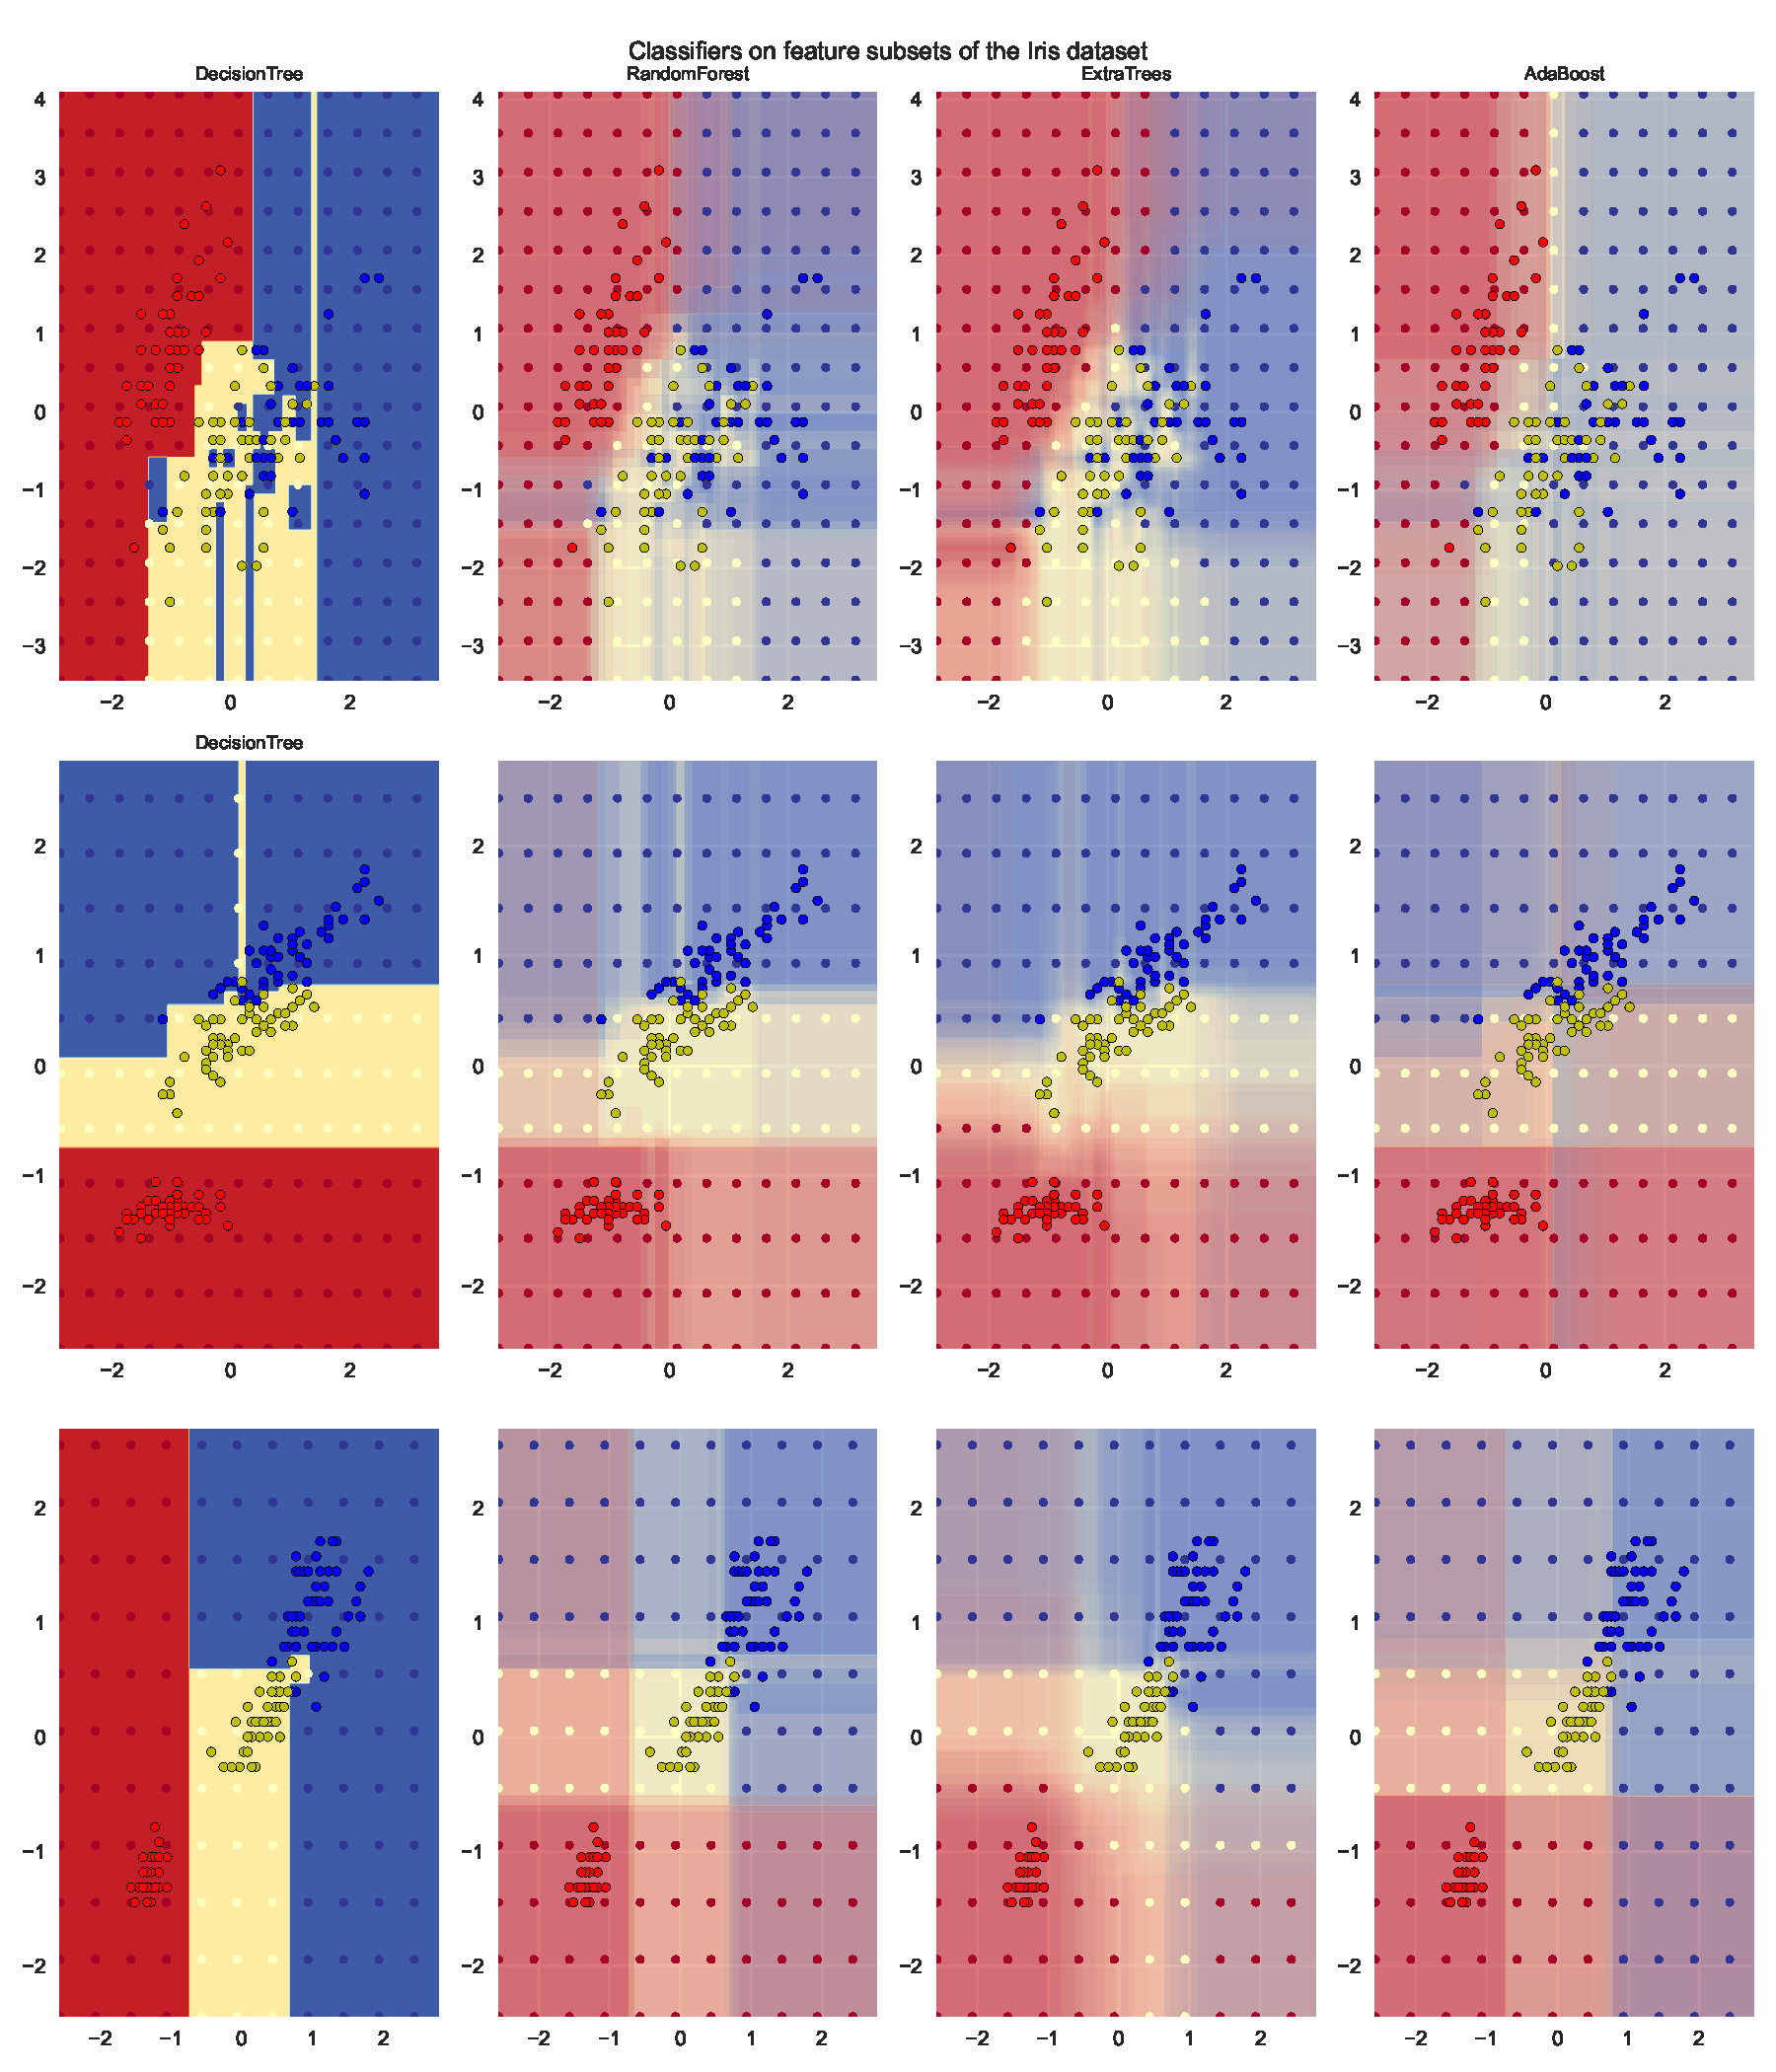
\includegraphics[width=14cm]{codeimage/code2}
	\caption{code2}
	\label{code2}
\end{figure}

\begin{PythonCode}\label{例3}
	\begin{Verbatim}[commandchars=\\\{\}]
\PY{c+c1}{\PYZsh{} 导入操作系统库}
\PY{k+kn}{import} \PY{n+nn}{os}
\PY{c+c1}{\PYZsh{} 更改工作目录}
\PY{n}{os}\PY{o}{.}\PY{n}{chdir}\PY{p}{(}\PY{l+s+sa}{r}\PY{l+s+s2}{\PYZdq{}}\PY{l+s+s2}{D:}\PY{l+s+s2}{\PYZbs{}}\PY{l+s+s2}{softwares}\PY{l+s+s2}{\PYZbs{}}\PY{l+s+s2}{applied statistics}\PY{l+s+s2}{\PYZbs{}}\PY{l+s+s2}{pythoncodelearning}\PY{l+s+s2}{\PYZbs{}}\PY{l+s+s2}{chap6}\PY{l+s+s2}{\PYZbs{}}\PY{l+s+s2}{sourcecode}\PY{l+s+s2}{\PYZdq{}}\PY{p}{)}
\PY{c+c1}{\PYZsh{} 导入基础计算库}
\PY{k+kn}{import} \PY{n+nn}{numpy} \PY{k}{as} \PY{n+nn}{np}
\PY{c+c1}{\PYZsh{} 导入绘图库}
\PY{k+kn}{import} \PY{n+nn}{matplotlib}\PY{n+nn}{.}\PY{n+nn}{pyplot} \PY{k}{as} \PY{n+nn}{plt}
\PY{c+c1}{\PYZsh{} 导入数据集工具}
\PY{k+kn}{from} \PY{n+nn}{sklearn}\PY{n+nn}{.}\PY{n+nn}{datasets} \PY{k+kn}{import} \PY{n}{load\PYZus{}diabetes}
\PY{c+c1}{\PYZsh{} 导入集成模型}
\PY{k+kn}{from} \PY{n+nn}{sklearn}\PY{n+nn}{.}\PY{n+nn}{ensemble} \PY{k+kn}{import} \PY{n}{GradientBoostingRegressor}
\PY{c+c1}{\PYZsh{} 导入均方误差工具}
\PY{k+kn}{from} \PY{n+nn}{sklearn}\PY{n+nn}{.}\PY{n+nn}{metrics} \PY{k+kn}{import} \PY{n}{mean\PYZus{}squared\PYZus{}error}
\PY{c+c1}{\PYZsh{} 导入数据集划分工具}
\PY{k+kn}{from} \PY{n+nn}{sklearn}\PY{n+nn}{.}\PY{n+nn}{model\PYZus{}selection} \PY{k+kn}{import} \PY{n}{train\PYZus{}test\PYZus{}split}
\PY{c+c1}{\PYZsh{} 导入绘图库中的字体管理包}
\PY{k+kn}{from} \PY{n+nn}{matplotlib} \PY{k+kn}{import} \PY{n}{font\PYZus{}manager}
\PY{c+c1}{\PYZsh{} 实现中文字符正常显示}
\PY{n}{font} \PY{o}{=} \PY{n}{font\PYZus{}manager}\PY{o}{.}\PY{n}{FontProperties}\PY{p}{(}\PY{n}{fname}\PY{o}{=}\PY{l+s+sa}{r}\PY{l+s+s2}{\PYZdq{}}\PY{l+s+s2}{C:}\PY{l+s+s2}{\PYZbs{}}\PY{l+s+s2}{Windows}\PY{l+s+s2}{\PYZbs{}}\PY{l+s+s2}{Fonts}\PY{l+s+s2}{\PYZbs{}}\PY{l+s+s2}{SimKai.ttf}\PY{l+s+s2}{\PYZdq{}}\PY{p}{)}
\PY{c+c1}{\PYZsh{} 使用seaborn风格绘图}
\PY{n}{plt}\PY{o}{.}\PY{n}{style}\PY{o}{.}\PY{n}{use}\PY{p}{(}\PY{l+s+s2}{\PYZdq{}}\PY{l+s+s2}{seaborn\PYZhy{}v0\PYZus{}8}\PY{l+s+s2}{\PYZdq{}}\PY{p}{)}
\PY{c+c1}{\PYZsh{} 加载数据集}
\PY{n}{diabetes} \PY{o}{=} \PY{n}{load\PYZus{}diabetes}\PY{p}{(}\PY{p}{)}
\PY{n}{X}\PY{p}{,} \PY{n}{y} \PY{o}{=} \PY{n}{diabetes}\PY{o}{.}\PY{n}{data}\PY{p}{,} \PY{n}{diabetes}\PY{o}{.}\PY{n}{target}
\PY{c+c1}{\PYZsh{} 划分数据集}
\PY{n}{X\PYZus{}train}\PY{p}{,} \PY{n}{X\PYZus{}test}\PY{p}{,} \PY{n}{y\PYZus{}train}\PY{p}{,} \PY{n}{y\PYZus{}test} \PY{o}{=} \PY{n}{train\PYZus{}test\PYZus{}split}\PY{p}{(}
    \PY{n}{X}\PY{p}{,} \PY{n}{y}\PY{p}{,} \PY{n}{test\PYZus{}size}\PY{o}{=}\PY{l+m+mf}{0.1}\PY{p}{,} \PY{n}{random\PYZus{}state}\PY{o}{=}\PY{l+m+mi}{13}
\PY{p}{)}
\PY{c+c1}{\PYZsh{} 设置一些参数}
\PY{n}{params} \PY{o}{=} \PY{p}{\PYZob{}}
    \PY{l+s+s2}{\PYZdq{}}\PY{l+s+s2}{n\PYZus{}estimators}\PY{l+s+s2}{\PYZdq{}}\PY{p}{:} \PY{l+m+mi}{500}\PY{p}{,}
    \PY{l+s+s2}{\PYZdq{}}\PY{l+s+s2}{max\PYZus{}depth}\PY{l+s+s2}{\PYZdq{}}\PY{p}{:} \PY{l+m+mi}{4}\PY{p}{,}
    \PY{l+s+s2}{\PYZdq{}}\PY{l+s+s2}{min\PYZus{}samples\PYZus{}split}\PY{l+s+s2}{\PYZdq{}}\PY{p}{:} \PY{l+m+mi}{5}\PY{p}{,}
    \PY{l+s+s2}{\PYZdq{}}\PY{l+s+s2}{learning\PYZus{}rate}\PY{l+s+s2}{\PYZdq{}}\PY{p}{:} \PY{l+m+mf}{0.01}\PY{p}{,}
    \PY{l+s+s2}{\PYZdq{}}\PY{l+s+s2}{loss}\PY{l+s+s2}{\PYZdq{}}\PY{p}{:} \PY{l+s+s2}{\PYZdq{}}\PY{l+s+s2}{squared\PYZus{}error}\PY{l+s+s2}{\PYZdq{}}\PY{p}{,}
\PY{p}{\PYZcb{}}
\PY{c+c1}{\PYZsh{} 构建模型}
\PY{n}{reg} \PY{o}{=} \PY{n}{GradientBoostingRegressor}\PY{p}{(}\PY{o}{*}\PY{o}{*}\PY{n}{params}\PY{p}{)}
\PY{c+c1}{\PYZsh{} 模型拟合}
\PY{n}{reg}\PY{o}{.}\PY{n}{fit}\PY{p}{(}\PY{n}{X\PYZus{}train}\PY{p}{,} \PY{n}{y\PYZus{}train}\PY{p}{)}
\PY{c+c1}{\PYZsh{} 预测}
\PY{n}{y\PYZus{}pred} \PY{o}{=} \PY{n}{reg}\PY{o}{.}\PY{n}{predict}\PY{p}{(}\PY{n}{X\PYZus{}test}\PY{p}{)}
\PY{c+c1}{\PYZsh{} 均方误差}
\PY{n}{mse} \PY{o}{=} \PY{n}{mean\PYZus{}squared\PYZus{}error}\PY{p}{(}\PY{n}{y\PYZus{}test}\PY{p}{,} \PY{n}{y\PYZus{}pred}\PY{p}{)}
\PY{n+nb}{print}\PY{p}{(}\PY{l+s+s2}{\PYZdq{}}\PY{l+s+s2}{The mean squared error (MSE) on test set: }\PY{l+s+si}{\PYZob{}:.4f\PYZcb{}}\PY{l+s+s2}{\PYZdq{}}\PY{o}{.}\PY{n}{format}\PY{p}{(}\PY{n}{mse}\PY{p}{)}\PY{p}{)}
\PY{c+c1}{\PYZsh{} 初始化测试集上的mse}
\PY{n}{test\PYZus{}score} \PY{o}{=} \PY{n}{np}\PY{o}{.}\PY{n}{zeros}\PY{p}{(}\PY{p}{(}\PY{n}{params}\PY{p}{[}\PY{l+s+s2}{\PYZdq{}}\PY{l+s+s2}{n\PYZus{}estimators}\PY{l+s+s2}{\PYZdq{}}\PY{p}{]}\PY{p}{,}\PY{p}{)}\PY{p}{,} \PY{n}{dtype}\PY{o}{=}\PY{n}{np}\PY{o}{.}\PY{n}{float64}\PY{p}{)}
\PY{c+c1}{\PYZsh{} 阶段性预测X\PYZus{}test}
\PY{k}{for} \PY{n}{i}\PY{p}{,} \PY{n}{y\PYZus{}pred} \PY{o+ow}{in} \PY{n+nb}{enumerate}\PY{p}{(}\PY{n}{reg}\PY{o}{.}\PY{n}{staged\PYZus{}predict}\PY{p}{(}\PY{n}{X\PYZus{}test}\PY{p}{)}\PY{p}{)}\PY{p}{:}
    \PY{c+c1}{\PYZsh{} 得到回归的mse}
    \PY{n}{test\PYZus{}score}\PY{p}{[}\PY{n}{i}\PY{p}{]} \PY{o}{=} \PY{n}{mean\PYZus{}squared\PYZus{}error}\PY{p}{(}\PY{n}{y\PYZus{}test}\PY{p}{,} \PY{n}{y\PYZus{}pred}\PY{p}{)}

\PY{n}{fig}\PY{p}{,} \PY{n}{ax} \PY{o}{=} \PY{n}{plt}\PY{o}{.}\PY{n}{subplots}\PY{p}{(}\PY{n}{figsize}\PY{o}{=}\PY{p}{(}\PY{l+m+mi}{6}\PY{p}{,} \PY{l+m+mi}{6}\PY{p}{)}\PY{p}{,} \PY{n}{tight\PYZus{}layout}\PY{o}{=}\PY{k+kc}{True}\PY{p}{)}
\PY{n}{ax}\PY{o}{.}\PY{n}{set\PYZus{}title}\PY{p}{(}\PY{l+s+s2}{\PYZdq{}}\PY{l+s+s2}{Deviance}\PY{l+s+s2}{\PYZdq{}}\PY{p}{)}
\PY{n}{ax}\PY{o}{.}\PY{n}{plot}\PY{p}{(}
    \PY{n}{np}\PY{o}{.}\PY{n}{arange}\PY{p}{(}\PY{n}{params}\PY{p}{[}\PY{l+s+s2}{\PYZdq{}}\PY{l+s+s2}{n\PYZus{}estimators}\PY{l+s+s2}{\PYZdq{}}\PY{p}{]}\PY{p}{)} \PY{o}{+} \PY{l+m+mi}{1}\PY{p}{,}
    \PY{n}{reg}\PY{o}{.}\PY{n}{train\PYZus{}score\PYZus{}}\PY{p}{,}
    \PY{l+s+s2}{\PYZdq{}}\PY{l+s+s2}{b\PYZhy{}}\PY{l+s+s2}{\PYZdq{}}\PY{p}{,}
    \PY{n}{label}\PY{o}{=}\PY{l+s+s2}{\PYZdq{}}\PY{l+s+s2}{Training Set Deviance}\PY{l+s+s2}{\PYZdq{}}\PY{p}{,}
\PY{p}{)}
\PY{n}{ax}\PY{o}{.}\PY{n}{plot}\PY{p}{(}
    \PY{n}{np}\PY{o}{.}\PY{n}{arange}\PY{p}{(}\PY{n}{params}\PY{p}{[}\PY{l+s+s2}{\PYZdq{}}\PY{l+s+s2}{n\PYZus{}estimators}\PY{l+s+s2}{\PYZdq{}}\PY{p}{]}\PY{p}{)} \PY{o}{+} \PY{l+m+mi}{1}\PY{p}{,} 
    \PY{n}{test\PYZus{}score}\PY{p}{,} \PY{l+s+s2}{\PYZdq{}}\PY{l+s+s2}{r\PYZhy{}}\PY{l+s+s2}{\PYZdq{}}\PY{p}{,} \PY{n}{label}\PY{o}{=}\PY{l+s+s2}{\PYZdq{}}\PY{l+s+s2}{Test Set Deviance}\PY{l+s+s2}{\PYZdq{}}
\PY{p}{)}
\PY{n}{ax}\PY{o}{.}\PY{n}{legend}\PY{p}{(}\PY{n}{loc}\PY{o}{=}\PY{l+s+s2}{\PYZdq{}}\PY{l+s+s2}{upper right}\PY{l+s+s2}{\PYZdq{}}\PY{p}{)}
\PY{n}{ax}\PY{o}{.}\PY{n}{set\PYZus{}xlabel}\PY{p}{(}\PY{l+s+s2}{\PYZdq{}}\PY{l+s+s2}{Boosting Iterations}\PY{l+s+s2}{\PYZdq{}}\PY{p}{)}
\PY{n}{ax}\PY{o}{.}\PY{n}{set\PYZus{}ylabel}\PY{p}{(}\PY{l+s+s2}{\PYZdq{}}\PY{l+s+s2}{Deviance}\PY{l+s+s2}{\PYZdq{}}\PY{p}{)}
\PY{n}{plt}\PY{o}{.}\PY{n}{show}\PY{p}{(}\PY{p}{)}
\PY{n}{fig}\PY{o}{.}\PY{n}{savefig}\PY{p}{(}\PY{l+s+s2}{\PYZdq{}}\PY{l+s+s2}{../codeimage/code3.pdf}\PY{l+s+s2}{\PYZdq{}}\PY{p}{)}
\end{Verbatim}

\begin{Verbatim}[commandchars=\\\{\}]
The mean squared error (MSE) on test set: 3041.0505
\end{Verbatim}
\end{PythonCode}

\begin{figure}
	\centering
	\includegraphics[width=14cm]{codeimage/code3}
	\caption{code3}
	\label{code3}
\end{figure}
